\section{Visualizing Linear Systems}
\label{sec:visualizing-linear-systems}

In this, rather informal, section, we present a way to visualize linear systems
in two and three variables and their solutions. Why two and three, you ask? The
number of variables in a linear equation determines the \emph{dimension} of the
\emph{geometric object} described by this equation. We shall soon provide the
necessary definitions to make rigorous sense of the sentence previous.
Intuitively, each variable represents a new `direction' we're allowed to move
in. Therefore, linear equations in two variables live in two-dimensional spaces
and linear equations in three variables occupy three dimensions.

Nonetheless, the equations themselves (if non-trivial) never describe objects of
the maximal possible dimension but of the dimension lower by one. This is
because they establish a relationship between the variables -- a relationship
where one variable grows entirely dependent on the rest, essentially `locking' a
single direction of movement. Think of it like this: a linear equation in two
variables is a sort of order, telling you that for every step forward you must
also make (say) two steps to the right, thereby rendering you unable to ever
walk in a direction different from the initial.

We proceed to show that the objects described by linear equations in two
variables are \emph{straight lines}. Said `objects described' are formally the
sets of points satisfying given equations. For instance, the object described by
the equation $3x + 2y = 4$ is the set
\[
 L \coloneqq \{(x,y) \in \R^2 \mid 3x + 2y = 4\}.
\]
Before we move on, we need establish an important fact. What is a \emph{straight
line} \textbf{exactly}? Wishing not to cheat and define straight line as the
object described by a linear equation, we employ a more geometric approach to
the definition. As we hope dear readers agree, a (one-dimensional) object is
\emph{straight} if moving along it requires `keeping the initial direction',
that is, always moving the same number of steps upward for a given number of
steps rightward, or vice versa. In other words, the \emph{ratio} between the
number of steps upward and rightward must remain constant. We encourage kind
readers to absorb that this particular property is what distinguishes
\emph{curved} objects from \emph{straight} ones.

\begin{figure}[ht]
 \centering
 \begin{tikzpicture}
  \tkzInit[xmin=-1,xmax=5,ymin=-1,ymax=2]
  \tkzDrawX
  \tkzDrawY

  \tkzDefPoints{0/0/A,2/1/B,1.5/0.75/C,3.5/1.75/D,3.5/0.75/E}
  \tkzDrawLine[color=BrickRed,thick,add=.5 and 1](A,B)
  \tkzDrawPoint[size=4,color=RoyalBlue](E)
  \tkzDrawSegments[dashed,thick,color=RoyalBlue](C,E D,E)
  \tkzDrawPoints[size=4,color=BrickRed](C,D)
  \tkzLabelPoint[above,color=BrickRed,xshift=-3mm,yshift=1mm](C){$(x_1,y_1)$}
  \tkzLabelPoint[above,color=BrickRed,xshift=-3mm,yshift=1mm](D){$(x_2,y_2)$}
  \tkzLabelSegment[right,color=RoyalBlue](D,E){$\Delta y = y_2 - y_1$}
  \tkzLabelSegment[below,color=RoyalBlue](C,E){$\Delta x = x_2 - x_1$}
 \end{tikzpicture}
 \caption{The `definition' of straightness. The ratio $\clb{\Delta y / \Delta
  x}$ must remain \textbf{constant}. It is habitually referred to as the
  \emph{slope} of the line.}
 \label{fig:straight-line}
\end{figure}

\myref{Figure}{fig:straight-line} inspires the following definition.

\begin{definition}{Straight line}{straight-line}
 An \textbf{infinite} subset $L \subseteq \R^2$ is called a \emph{straight line}
 if for all triples of points $(x_1,y_1)$, $(x_2,y_2)$, $(x_3,y_3) \in L$ it
 holds true that either
 \begin{equation}
  \label{eq:straight-line}
  \frac{y_2 - y_1}{x_2 - x_1} = \frac{y_3 - y_2}{x_3 - x_2},
 \end{equation}
 or $x_1 = x_2 = x_3$ (a vertical line).
\end{definition}

We proceed to show that the all the points in the plane satisfying a linear
equation form a \hyperref[def:straight-line]{straight line}. This is exceedingly
easy. Suppose we have three solutions $(x_1,y_1),(x_2,y_2)$ and $(x_3,y_3)$
satisfying the equation $ax + by = c$, where $a,b,c \in \R$ and at least one of
$a$, $b$ is not zero. In other words, we have $ax_i + by_i = c$ for $i \in
\{1,2,3\}$.

We've had to exclude the case $a = b = 0$ because the set of solutions of the
linear equation $0 = c$ is never a straight line. If $c \neq 0$, it is empty,
and if $c = 0$, it equals $\R^2$.

Assume first that $b = 0$. Then, $x_i = c / a$ and so $x_1 = x_2 = x_3$. Hence,
in this case, the set of solutions is indeed a straight line.

In case $b \neq 0$, we may rearrange
\[
 y_i = \frac{c - ax_i}{b}.
\]
Plugging this into~\eqref{eq:straight-line} gives
\begin{equation}
 \label{eq:straight-line-sub}
 \frac{(c - ax_2) - (c - ax_1)}{b(x_2 - x_1)} = \frac{(c - ax_3) - (c -
 ax_1)}{b(x_3 - x_1)}.
\end{equation}
Simple calculation yields
\[
 \frac{(c - ax_2) - (c - ax_1)}{b(x_2 - x_1)} = \frac{a(x_1 - x_2)}{b(x_2 -
 x_1)} = - \frac{a}{b}
\]
and similarly for $(y_3 - y_1) / (x_3 - x_1)$. Hence, both sides
of~\eqref{eq:straight-line-sub} equal $-a / b$ and the proof is complete.

\subsection{Two-dimensional Linear Systems}
\label{ssec:two-dimensional-linear-systems}

We dedicate this section to the visualization of linear systems in two variables
and their solutions. As already established, a linear equation in two variables
represents a \hyperref[def:straight-line]{straight line}. A solution to a linear
system in two variables is a pair of real numbers (equivalently, a point in the
real plane) which lies on every straight line determined by the equations of the
system. Simply put, the solution of a linear system in two variables is the
\emph{intersection} of all objects described by its equations.

An `ideal' linear system in two variables contains two linear equations
describing distinct lines. One such system is
\[
 \begin{array}{r c r c r}
  2x & - & y & = & 1\\
  x & + & y & = & 2
 \end{array}
\]
with solution $(1,1)$ and whose visual depiction is provided in
\myref{figure}{fig:well-determined-system}.

\begin{figure}[ht]
 \centering
 \begin{tikzpicture}
  \tkzInit[xmin=-1,xmax=5,ymin=-1,ymax=2]
  \tkzDrawX
  \tkzDrawY
  \tkzDefPoints{0/0/o,1/1/i,0.5/0/a,2/0/b}
  \tkzDrawLine[color=RoyalBlue,thick,add=0.8 and 1.3](a,i)
  \tkzDrawLine[color=ForestGreen,thick,add=0.8 and 1.3](b,i)

  \tkzDefPoints{1/0/x,0/1/y}
  \tkzDrawPoint[size=6,color=BrickRed](i)
  \tkzLabelPoint[below](x){$1$}
  \tkzLabelPoint[left](y){$1$}
  \tkzLabelPoint[right=2mm,color=BrickRed](i){$(1,1)$}
  \tkzDrawSegments[dashed,thick,color=BrickRed](i,x i,y)
  \tkzDrawPoints[size=4](x,y)
 \end{tikzpicture}

 \caption{Well-determined linear system in two variables with solution
 $\clr{(1,1)}$.}
 \label{fig:well-determined-system}
\end{figure}

An easily proven fact (which we shall eventually prove in greater generality)
that follows immediately from the geometric view reads that a linear system in
two variables with two \emph{distinct} linear equations always has a solution --
the intersection point of the corresponding lines.

A linear system in two variables can only be underdetermined should it feature
just one non-trivial linear equation (or, equivalently, many identical linear
equations). 

\subsection{Three-dimensional Linear Systems}
\label{ssec:three-dimensional-linear-systems}

Stepping up the game a little, we're taking a look at linear systems in three
variables. Just as a linear equations in two variables are lines in the real
plane, linear equations in three variables depict geometric objects called
`planes' in the three-dimensional real space, $\R^3$. They form the last class
of linear systems that can be efficiently visualized; with linear systems in
more variables being generally out of our perceptive reach.

Planes are the \emph{straight} objects in three-dimensional kind of sense. They
lock one direction of movement by making one variable wholly dependent on the
other two. An illustration is provided in \myref{figure}{fig:plane}.

\begin{figure}[ht]
 \centering
 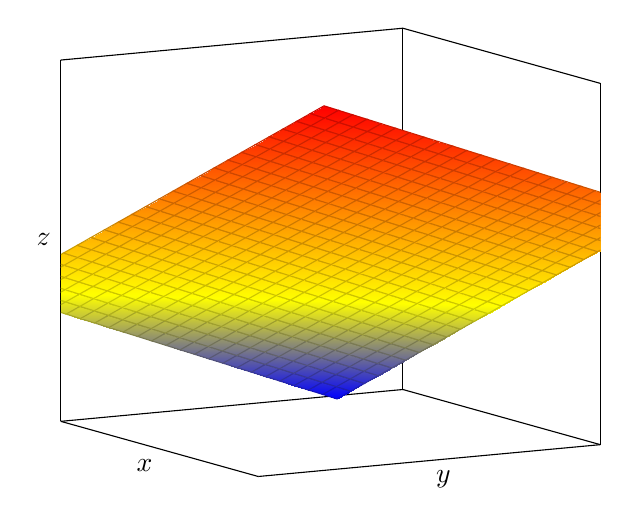
\begin{tikzpicture}
  \begin{axis}[
   view={60}{10},
   xlabel={$x$},
   ylabel={$y$},
   zlabel={$z$},
   zlabel style={rotate=90},
   xtick=\empty,
   ytick=\empty,
   ztick=\empty,
   xmin=-3,
   xmax=3,
   ymin=-5,
   ymax=5
  ]
   \addplot3[
    surf,
    colormap/hot,
    shader=faceted interp,
    ]({x}, {y}, {(2*x - y + 3) / 3});
  \end{axis}
 \end{tikzpicture}

 \caption{A \clb{plane} defined by the equation $2x - y - 3z = -3$.}
 \label{fig:plane}
\end{figure}

An \emph{underdetermined} system in three variables can contain either one or
two linear equations. In the former case, only one variable is dependent on the
other two -- we shall often call the independent variables by names such as
\emph{free variables} or \emph{parameters}. Both these names signify that a
substitution of any pair of real numbers in lieu of the two \emph{free
variables} yields a solution of the system.

For instance, the linear equation in \myref{figure}{fig:plane} is effectively a
linear system in three variables. We can choose any of the three variables to be
dependent and leave the other two free, giving thus three different descriptions
of \emph{the same} solution set. The following
equation~\eqref{eq:three-vars-one-eq} shows all of them with the chosen
dependent variable written on the left in typewriter font.
\begin{equation}
 \label{eq:three-vars-one-eq}
 \begin{array}{r l}
  \mathtt{x:} & \left\{ \left( \frac{y + 3z - 3}{2}, y, z \right) \mid y,z \in \R
  \right\}\\[1em]
  \mathtt{y:} & \left\{ \left( x, 2x - 3z + 3, z \right) \mid x,z \in \R
  \right\}\\[1em]
   \mathtt{z:} & \left\{ \left( x, y, \frac{2x - y + 3}{3} \right) \mid x,y \in
   \R \right\}
 \end{array}
\end{equation}

Linear systems in three variables and two equations are also underdetermined.
Geometrically, they correspond to arrangements of two planes in space. Those two
planes can either be parallel -- leading to the system having no solution -- or
not -- intersecting in a straight line describable as a set of triples with
exactly one free variable. In a case similar to two-dimensional linear systems,
putting the system in question into echelon form \emph{can} reveal (albeit not
always) its geometric nature.

Indeed, consider the system
\begin{equation}
 \label{eq:two-parallel-planes}
 \begin{array}{r c r c r c r}
  x & - & y & + & 2z & = & 2\\
  2x & - & 2y & + & 4z & = & 9
 \end{array}.
\end{equation}
Subtracting $\mathtt{II - 2 \cdot I}$ produces
\[
 \begin{array}{r c r c r c r}
  x & - & y & + & 2z & = & 2\\
    &   &   &   &  0 & = & 5
 \end{array},
\]
clearly a system with no solution. Subsequently, the two corresponding planes
are parallel to each other. See them depicted in
\myref{figure}{fig:two-parallel-planes}.

\begin{figure}[ht]
 \centering
 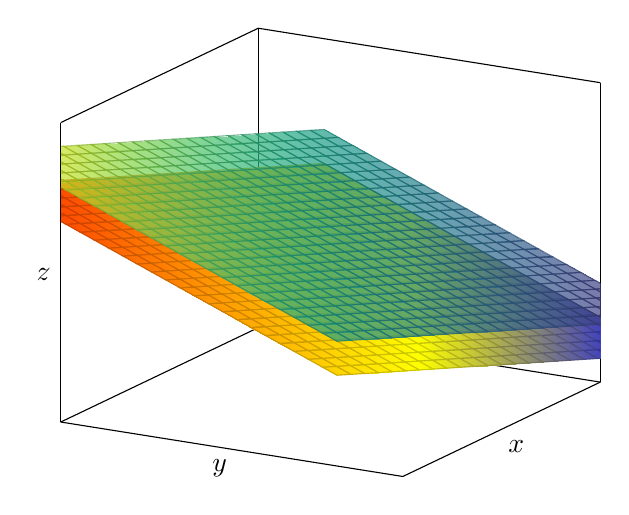
\begin{tikzpicture}
  \begin{axis}[
   view={-60}{20},
   xlabel={$x$},
   ylabel={$y$},
   zlabel={$z$},
   zlabel style={rotate=90},
   xtick=\empty,
   ytick=\empty,
   ztick=\empty,
   xmin=-3,
   xmax=3,
   ymin=-5,
   ymax=5
  ]
   \addplot3[
    surf,
    colormap/hot,
    shader=faceted interp,
   ]({x}, {y}, {(2 - x + y) / 2});
   \addplot3[
    surf,
    colormap/viridis,
    shader=faceted interp,
    opacity=0.7,
   ]({x}, {y}, {(9 - 2*x + 2*y) / 4});
  \end{axis}
 \end{tikzpicture}

 \caption{The two parallel planes from the
 system~\eqref{eq:two-parallel-planes}.}
 \label{fig:two-parallel-planes}
\end{figure}

A system of two non-parallel planes is presented below.
\begin{equation}
 \label{eq:two-non-parallel-planes}
 \begin{array}{r c r c r c r}
  x & - & y & + & 2z & = & 2\\
  2x & + & 3y & - & z & = & -1
 \end{array}
\end{equation}
By subtracting, once again, $\mathtt{II - 2 \cdot I}$, we put into the following
echelon form.
\[
 \begin{array}{r c r c r c r}
  x & - & y & + & 2z & = & 2\\
    &   & 5y & - & 5z & = & -5
 \end{array}
\]
The algorithm of Gauss-Jordan elimination limits our choice of free variables to
the ones left in the last row. We are hence to set either $y$ or $z$ loose while
caging the latter. Custom dictates to label all variables but the first of the
last row as \emph{parameters}, making $z$ the victor. The rest is just
back-substitution. We calculate $y = z - 1$ and substitute into the first
equation to receive
\[
 x - (z - 1) + 2z = 2, \quad \text{hence} \quad x = 1 - z.
\]
It follows that \emph{one possible} description of the solution set of the
system~\eqref{eq:two-non-parallel-planes} is
\[
 \left\{ (1 - z, z - 1, z) \mid z \in \R\right\}.
\]
See it depicted in \myref{figure}{fig:two-non-parallel-planes}.
\begin{figure}[ht]
 \centering
 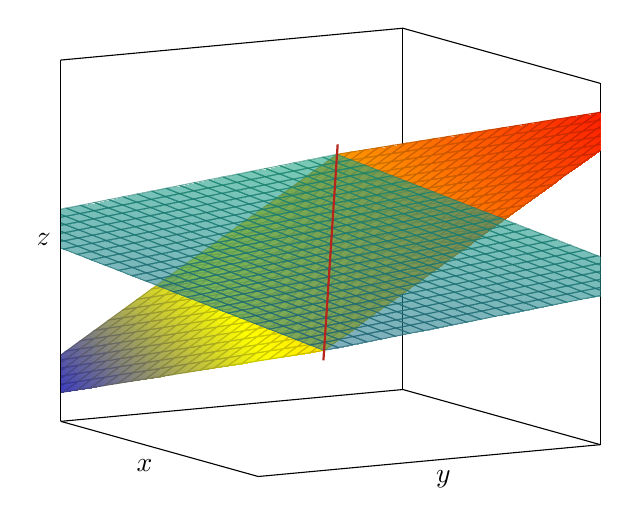
\begin{tikzpicture}
  \begin{axis}[
   view={60}{10},
   xlabel={$x$},
   ylabel={$y$},
   zlabel={$z$},
   zlabel style={rotate=90},
   xtick=\empty,
   ytick=\empty,
   ztick=\empty,
   xmin=-3,
   xmax=3,
   ymin=-5,
   ymax=5
  ]
   \addplot3[
    surf,
    colormap/hot,
    shader=faceted interp,
   ]({x}, {y}, {2*x + 3*y + 1});
   \addplot3[
    surf,
    colormap/viridis,
    shader=faceted interp,
    opacity=0.6
   ]({x}, {y}, {(2 - x + y) / 2});
  \addplot3[
   color=BrickRed,
   thick,
   smooth
  ]({x},{-x},{1-x});
  \end{axis}
 \end{tikzpicture}

 \caption{The two non-parallel planes from the
 system~\eqref{eq:two-non-parallel-planes} and their \clr{intersection}.}
 \label{fig:two-non-parallel-planes}
\end{figure}

Reaching the apex of `ideal' linear systems in three variables and three
equations, we stop to ponder the number of arrangements of three planes in
three-dimensional space. There are two obvious ones:
\begin{enumerate}
 \item All three planes are parallel to each other.
 \item Only two planes are parallel to each other.
\end{enumerate}
Corresponding to (1), resp. (2), is a linear system with two equations, resp.
one equation, with no solution.

As an example, consider the system
\begin{equation}
 \label{eq:two-parallel-one-not}
 \begin{array}{r c r c r c r}
  -x & + & 2y & - & z & = & 4\\
  x & - & 6y & + & z & = & 1\\
  x & - & 2y & + & z & = & 3
 \end{array}.
\end{equation}
Its echelon form looks like this:
\[
 \begin{array}{r c r c r c r}
  -x & + & 2y & - & z & = & 4\\
     & & -4y & & & = & 5\\
     & & & & 0 & = & 7
 \end{array}.
\]
Clearly, the third equation has no solution while the second does. This
particular system's geometrical interpretation aligns with case (2) above. It is
shown in \myref{figure}{fig:two-parallel-one-not}.
\begin{figure}[ht]
 \centering
 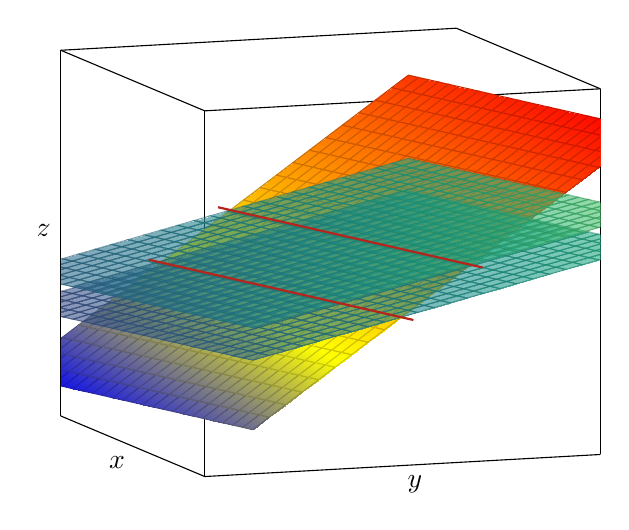
\begin{tikzpicture}
  \begin{axis}[
   view={110}{-10},
   xlabel={$x$},
   ylabel={$y$},
   zlabel={$z$},
   zlabel style={rotate=90},
   xtick=\empty,
   ytick=\empty,
   ztick=\empty,
   xmin=-3,
   xmax=3,
   ymin=-5,
   ymax=5
  ]
   \addplot3[
    surf,
    colormap/hot,
    shader=faceted interp
   ]({x}, {y}, {-x + 6*y + 1});
   \addplot3[
    surf,
    colormap/viridis,
    shader=faceted interp,
    opacity=0.6
   ]({x}, {y}, {-x + 2*y - 4});
   \addplot3[
    surf,
    colormap/viridis,
    shader=faceted interp,
    opacity=0.6
   ]({x}, {y}, {-x + 2*y + 3});
   \addplot3[
    color=BrickRed,
    thick,
    smooth
   ]({x},{1/2},{4-x});
   \addplot3[
    color=BrickRed,
    thick,
    smooth
   ]({x},{-5/4},{-x - 13/2});
  \end{axis}
 \end{tikzpicture}

 \caption{Depiction of the system~\eqref{eq:two-parallel-one-not}.}
 \label{fig:two-parallel-one-not}
\end{figure}

Finally, there are three other possible arrangements of three planes in space:
\begin{enumerate}
 \setcounter{enumi}{2}
 \item non-parallel planes that fail to have a common intersection (the
  so-often-called `tent' configuration);
 \item non-parallel planes that meet in a single point;
 \item non-parallel planes that meet in a single line.
\end{enumerate}
Of course, as always, the echelon form of a linear system can be used to
distinctively label it as any of these cases. For example, the echelon form of
the system
\begin{equation}
 \label{eq:tent}
 \begin{array}{r c r c r c r}
  x & + & 2y & - & z & = & -1\\
  2x & - & 3y & + & 2z & = & 4\\
  -x & + & 5y & - & 3z & = & 10
 \end{array}
\end{equation}
can easily be computed to be
\[
 \begin{array}{r c r c r c r}
  x & + & 2y & - & z & = & -1\\
    & & -7y & + & 4z & = & 6\\
    & & & & 0 & = & 15
 \end{array}.
\]


